%!TEX root = ../main.tex
\subsection{\acs{ui} Backend}
\thomas{ensure that they actually do state that this is a requirement}
The requirements state that it should be simple to add additional sensors to the system.
Adding a sensor includes creating a way of easily accessing and showing the data on the observing system.
This section will explain the design of the backend that will provide this functionality.

\subsubsection*{Data Format}
Depending on the author of the data (which node produced the data) the data may be inherently different.
The interpretation of data is therefore not uniform across the entire system.
For this reason, it is necessary to create a system that is agnostic with respect to the type and amount of data being handled.
In section \ref{sub:CAN_protocol} a description of the node and message identification system is given.
The NodeID and MSGtype identifiers are decided by the implementer and together they provide a unique, 11 bit identifier, the Message ID, for the type of data in the message.
Since the Message ID is capable of uniquely identifying the data, it will be used in storing the data.
Additionally each message will be associated with a four byte timestamp.
This timestamp is given as the time in milliseconds since startup and is associated with message type <type>. \thomas{insert correct message type}
\thomas{We need to agree on a way to write nodeid,msgid,msgtype throughout the report}

\subsubsection*{Backend Architecture}
An overview of the functionality can be seen in figure \ref{fig:backendconcept}.
As can be seen, this architecture provides the link between the receiving program (socat) and a potential \acs{gui}.
Upon receiving a message from the go-kart, socat will pipe the raw message to the interpreter.
The interpreter will proceed to extract the message id, the timestamp and the data.
These are then put into a fifo buffer which will contain the latest 1024 data points for a given message id.
\thomas{Why 1024? An arbitrary number that needs some sort of explanation..}
The backend is a collection of functions which provide an API for the UI layer. 

\begin{figure}
	\includegraphics[width=\linewidth]{graphics/backend_concept}
	\caption[Overview of the backend functionality.]{Overview of the backend functionality. 
	Messages are received over wifi from the go-kart. 
	An interpreter reads the message to determine the MessageID (MSGID), timestamp (T) and the data. 
	All information is made available to a \acs{gui} through the backend.}
	\label{fig:backendconcept}
\end{figure}

\begin{figure}[H]
	\missingfigure{Backend Class Diagram}
	%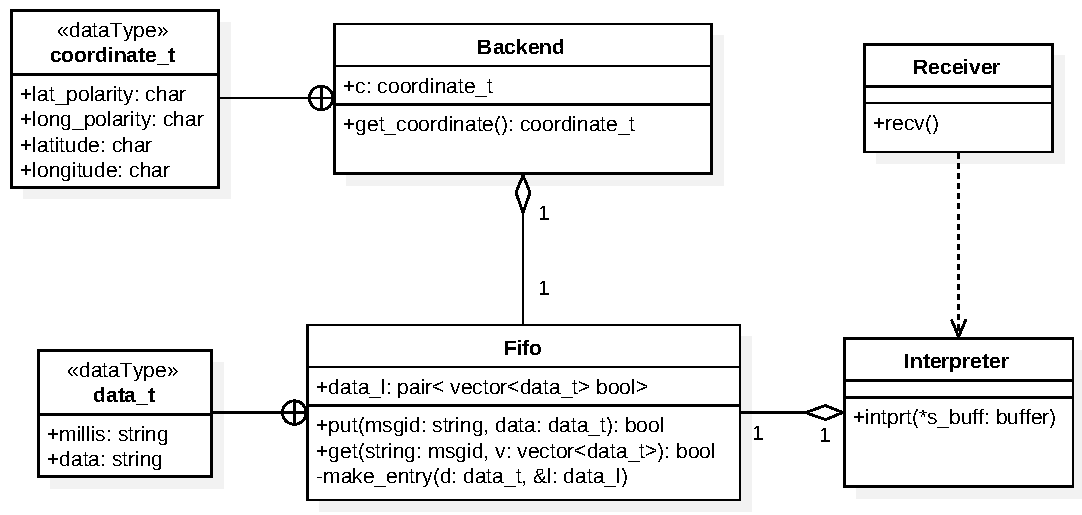
\includegraphics[width=\linewidth]{graphics/backend_class_diagram}
	\caption[Backend class diagram.]{Classdiagram of the backend.}
	\label{fig:backendclass}
\end{figure}

From \ref{fig:backendconcept}, a class diagram has been created.
This can be seen on figure \ref{fig:backendclass}.
Four classes are created, each of which will be explained in more detail below

\paragraph*{\texttt{receiver}}~\\
This class is run in a separate thread.
It continuously listens to std::io, waiting for input from the go-kart.
Upon receiving a message, it is put into a buffer maintained by interpreter.
\paragraph*{\texttt{interpreter}}~\\
As mentioned, this class holds a message buffer, shown in code \ref{code:msgbuffer}.
Whenever a message is put in the buffer, it is split into its three components, a 10 bit message id, a 4 byte timestamp and an data of arbitrary length.
On figure \ref{fig:backendmsg} is a depiction of a message.
\begin{figure}[H]
	\missingfigure{Backend Message (msgid/timestamp/data)}
	%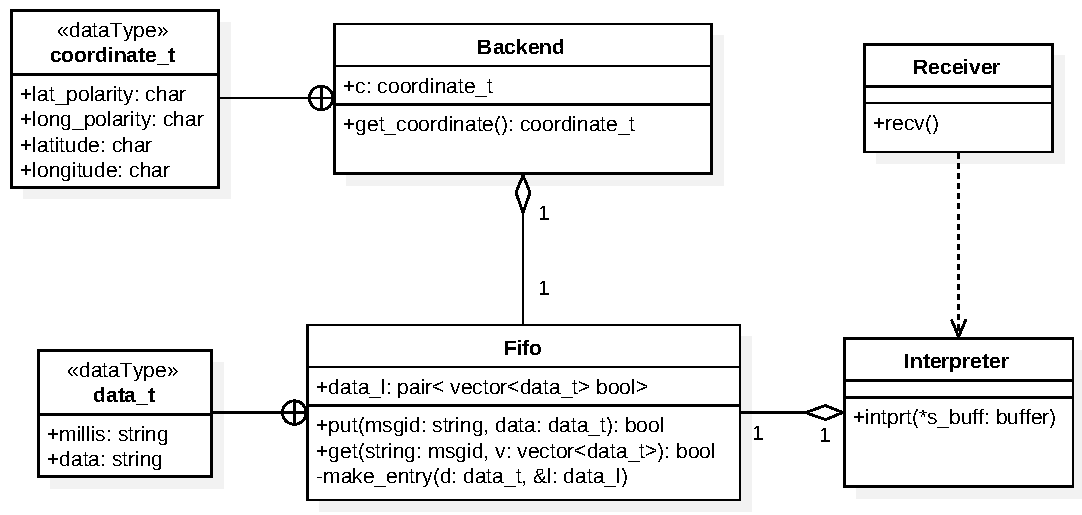
\includegraphics[width=\linewidth]{graphics/backend_class_diagram}
	\caption[Wifi Message.]{Depiction of the message sent over wifi.}
	\label{fig:backendmsg}
\end{figure}

Once split, the information is stored using the put function 
\begin{lstlisting}[caption=Buffer for holding incomming messages,label=code:msgbuffer]
struct buffer 
{
  std::vector<std::string> strings;
  std::mutex mutex;
};
\end{lstlisting}